\begin{figure}
  \centering
  \def\W{1.25}
  \def\H{1.25}
  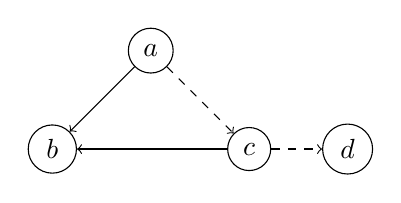
\begin{tikzpicture}
    \tikzset{
      host/.style={draw,circle}
    }
    \node[host] (a) at (0,\H) {$a$};
    \node[host] (b) at (-\W,0) {$b$};
    \node[host] (c) at (\W,0) {$c$};
    \node[host] (d) at (2*\W,0) {$d$};

    \path[->] (a) edge (b) edge[dashed] (c);
    \path[->] (c) edge (b) edge[dashed] (d);
  \end{tikzpicture}
  \caption{شبکه مثال لیست سیاه}
  \label{fig:blacklist-network}
\end{figure}